\section{Experiments}
\label{sec:experiments}

\subsection{Experimental Setup}

\paragraph{Datasets.}
\textbf{DAD}~\citep{ref4}: 1,750 dashcam videos (620 accident,
1,130 non-accident) from six Taiwanese cities, split 1,280/450
train/test. Videos are 5\,s at 20\,fps (100 frames).
\textbf{A3D}~\citep{liao2024crash}: 1,199 videos (960/239) at 10\,fps,
100 frames, spanning diverse East Asian urban accident types.

\paragraph{Metrics.}
\textbf{AP}: area under the precision-recall curve.
\textbf{mTTA}: mean lead time between first issued alert and annotated
accident onset over correctly anticipated positives.
\textbf{TTA@R80} / \textbf{P@R80}: TTA and precision at 80\% recall.

\paragraph{Implementation details.}
VGG16~\citep{ref31} ROI features ($D{=}4096$, $N{=}19$ objects per frame).
For the full historical vocabulary we use $K{=}837$ concepts; for discovered
ontologies, $K$ is the size of the corresponding compact concept set.
AdamW with learning rate $3{\times}10^{-4}$, cosine decay, batch size 16,
and a 150-epoch schedule with 15 epochs of Actor--Critic warmup followed by a
20-epoch CBM ramp in the shared comparison runs. For DAD, our strongest current
submission result additionally uses a lightweight curriculum-stabilized variant
that delays the concept loss in the earliest stage before gradually ramping in
concept supervision. This improves stability on DAD while keeping the test
protocol and model family unchanged. For concept-set comparison experiments, we
keep the training recipe fixed and vary only the ontology source and concept
count, allowing us to attribute changes in performance to the semantic
interface rather than to optimizer choices.

\paragraph{Result reporting protocol.}
We separate \emph{canonical headline runs} from \emph{controlled support analyses},
but we do not select checkpoints by test-set performance. For each reported
training line, the paper uses a pre-specified evaluation snapshot: either the
final training epoch under the stated schedule or a synchronized fixed epoch
used consistently across seeds for robustness reporting. Ontology comparison,
ablation, robustness, and intervention blocks are therefore interpreted as
separate analyses under fixed protocols rather than as a pool from which the
best test result is chosen. In brief: Table~\ref{tab:dad} uses the DAD
curriculum headline line; Table~\ref{tab:a3d} uses the shared A3D headline
line; Table~\ref{tab:ablation} uses a controlled support protocol; and
Table~\ref{tab:concept_sets} uses a shared-launcher ontology comparison.
This separation matters because it prevents historical runs, ontology-search
runs, and archived intervention assets from being mistaken for one unified
benchmark line. It also clarifies how to read the DAD robustness paragraph:
the 68.19\% AP headline number is a canonical single-run endpoint under the
curriculum-stabilized schedule, whereas the 55--56\% AP figures are
synchronized fixed-epoch diagnostics across three clean seeds. The latter are
therefore not intended as direct replacements for the headline line; they are a
checkpoint-sensitivity diagnostic showing that DAD remains materially more
fragile than A3D under clean synchronized evaluation.

\begin{table}[t]
\caption{Main-paper protocol map. This table gives a concise reading key for the main result blocks: recipe family, checkpoint rule, seed count, and which score source defines the reported alert timing.}
\label{tab:protocol_map_main}
\centering\small
\resizebox{\linewidth}{!}{%
\begin{tabular}{p{0.20\linewidth}p{0.17\linewidth}p{0.18\linewidth}ccc}
\toprule
Paper item & Recipe family & Checkpoint rule & Seeds & Score source & Role \\
\midrule
Table~\ref{tab:dad} & DAD curriculum-stabilized & canonical single-run endpoint & 1 & classifier & headline DAD \\
Table~\ref{tab:a3d} & shared default line & canonical single-run endpoint & 1 & classifier & headline A3D \\
Table~\ref{tab:concept_sets} & shared-launcher ontology comparison & one completed run per ontology/data pair & 1 each & classifier & ontology operating-point analysis \\
Table~\ref{tab:trigger_compare} & representative support checkpoints & matched checkpoint re-evaluation & 1 each & classifier / actor & score-source comparison \\
Table~\ref{tab:ablation} & controlled support protocol & fixed support line & 1 & classifier & component isolation \\
DAD robustness paragraph & clean curriculum family & synchronized epochs 25/30 & 3 & classifier & checkpoint-sensitivity diagnostic \\
\bottomrule
\end{tabular}%
}
\end{table}

\paragraph{Pseudo-label sensitivity.}
We also audited the top-$m$ CLIP pseudo-label recipe on 120 sampled DAD frames
from the paper ontology. The main takeaway is that top-3 is a reasonable
middle ground: top-1 is too concentrated (1.00 concept family per frame on
average), while top-10 becomes much more diffuse (5.20 families per frame).
Top-3 yields 2.36 families per frame on average, broadening the supervision
signal without making it overly dense. We therefore retain top-3 in the main
training recipe as a pragmatic compromise rather than as a claim of exact
semantic calibration.

\subsection{Interpretability Taxonomy of Prior Work}

\begin{table}[t]
\caption{Interpretability comparison. \textbf{WHY}: intrinsic concept
explanation. \textbf{WHEN}: intrinsic alert-timing explanation.
\method{} provides both within a single unified model.}
\label{tab:interp_comparison}
\centering\small
\begin{tabular}{lcccc}
\toprule
Method & WHY & WHEN & Intrinsic? & Params\\
\midrule
DSA-RNN~\citep{ref4}        & \texttimes & \texttimes & -- & 12M\\
DRIVE~\citep{ref2}          & Grad-CAM & \texttimes & post-hoc & 31M\\
DSTA~\citep{ref17}          & \texttimes & \texttimes & -- & 180M\\
DAA-GNN~\citep{ref32}       & \texttimes & \texttimes & -- & 183M\\
W3AL~\citep{liao2024and}    & \texttimes & verbal & post-hoc & 7B\\
CRASH~\citep{liao2024crash} & \texttimes & \texttimes & -- & 26M\\
CCAF-Net~\citep{liu2025ccaf}& \texttimes & \texttimes & -- & 191M\\
LATTE~\citep{ZHANG2025103173}& \texttimes & \texttimes & -- & 45M\\
\midrule
\textbf{\method{} (Ours)} & \textbf{837 concepts} &
  \textbf{AC policy} & \textbf{\checkmark} & \textbf{30M}\\
\bottomrule
\end{tabular}
\end{table}

Table~\ref{tab:interp_comparison} highlights a clear gap: prior work rarely
provides both WHY and WHEN interpretability intrinsically.
DRIVE's Grad-CAM is computed after prediction and carries no concept
structure; W3AL requires a 7B LLM and produces verbal localisation.
\method{} closes the representational gap architecturally with only 30M
parameters, while our current empirical evidence is strongest on the WHY layer,
on controlled timing improvements, and on the concept-conditioned timing
formulation rather than on a fully verified policy-level intervention story.

\subsection{Main Results on DAD}

\begin{table}[t]
\caption{DAD results. We separate intrinsically or explicitly interpretable methods from strong non-interpretable references. The goal of this table is not to claim the highest overall DAD score, but to position \method{} as a competitive intrinsically interpretable method while preserving a fair view of the broader leaderboard.}
\label{tab:dad}
\centering\small
\begin{tabular}{lcccc}
\toprule
Method & Venue & AP$\uparrow$ & mTTA$\uparrow$ & Interp.\\
\midrule
DSA-RNN~\citep{ref4}        & ACCV'16 & 38.1\% & 2.05s & \texttimes\\
DRIVE~\citep{ref2}          & ICCV'21 & 58.4\% & 2.31s & post-hoc\\
DSTA~\citep{ref17}          & TITS'22 & 56.1\% & 3.66s & \texttimes\\
Graph$^2$~\citep{ref36}     & WACV'24 & 64.8\% & 2.98s & \texttimes\\
DAA-GNN~\citep{ref32}       & PR'24 & 75.2\% & 1.59s & \texttimes\\
W3AL~\citep{liao2024and}    & MM'24 & 69.2\% & -- & verbal\\
CRASH~\citep{liao2024crash} & MM'24 & 65.3\% & 1.75s & \texttimes\\
\midrule
\method{} (Ours) & -- & 68.19\% & 1.75s & WHY+WHEN\\
\midrule
$\dagger$ CCAF-Net & -- & 81.3\% & 4.15s & \texttimes\\
$\dagger$ LATTE & -- & 89.7\% & 4.49s & \texttimes\\
\bottomrule
\end{tabular}
\end{table}

\method{} achieves 68.19\% AP and 1.75s mTTA, which places it in a
meaningful operating region for interpretable accident anticipation under the
current DAD headline protocol. This number should be read as the endpoint of
one canonical curriculum-stabilized line, not as a claim that DAD performance
is seed-stable at that level under synchronized clean-seed evaluation. The
paper therefore reports the lower 55--56\% synchronized multi-seed diagnostics
explicitly as a robustness check rather than obscuring the gap. The result is
not presented as the global DAD leaderboard winner; instead, its significance
is that it combines competitive predictive quality with a structured WHY layer
and a concept-conditioned timing formulation. Compared with DRIVE, it improves
AP by 9.8 points while replacing post-hoc explanation with a structured
concept-and-policy decomposition.

The non-interpretable references in Table~\ref{tab:dad} remain important
context, because they show how far the absolute DAD frontier has moved. Rather
than obscuring that gap, we make it explicit: the present contribution is that
\method{} occupies a substantially stronger interpretability/performance point
than prior interpretable or explanation-oriented alternatives, while preserving
small-model efficiency and a semantically auditable decision pathway.

\paragraph{Multi-seed robustness (DAD, curriculum line).}
To quantify checkpoint sensitivity in the curriculum-stabilized DAD line, we
launched three clean seeds ($7/43/123$) under the same configuration and
reported synchronized fixed-epoch checkpoints rather than per-seed best test
snapshots. At epoch~25, the three-seed aggregate is
$\text{AP}=56.39\%\pm3.46$ and $\text{mTTA}=2.40\pm0.05$~s
(mean$\pm$std; AP std in absolute points), with
$\text{TTA@R80}=3.11\pm0.03$~s and $\text{P@R80}=0.447\pm0.004$.
At epoch~30, the aggregate is
$\text{AP}=55.16\%\pm3.63$ and $\text{mTTA}=2.49\pm0.09$~s,
with $\text{TTA@R80}=3.17\pm0.06$~s and $\text{P@R80}=0.447\pm0.009$.
We report these synchronized checkpoints as a stability diagnostic rather than
as a replacement for the canonical single-run table entry. Their role is to
show that DAD remains checkpoint-sensitive and that the paper is explicit about
that variance, not to optimize over test checkpoints after the fact.
Importantly, these synchronized summaries still do not establish DAD hard-case
symmetry: failure behavior remains uneven across scenario types in the current
evidence package, so symmetry should be treated as an open validation target
rather than as a solved property.

\subsection{Main Results on A3D}

\begin{table}[t]
\caption{A3D results. \method{} improves mTTA over CRASH while CRASH retains the highest AP among the methods listed here. $\Delta$mTTA vs.\ CRASH~\citep{liao2024crash}.}
\label{tab:a3d}
\centering\small
\begin{tabular}{lccccc}
\toprule
Method & AP$\uparrow$ & mTTA$\uparrow$ & TTA@R80$\uparrow$ & P@R80$\uparrow$ & Interp.\\
\midrule
CRASH~\citep{liao2024crash} & 96.0\% & 4.27s & -- & -- & \texttimes\\
W3AL~\citep{liao2024and}    & 92.4\% & 4.52s & -- & -- & verbal\\
\midrule
\method{} & 93.4\% & 4.90s & 4.89s & 0.9067 & WHY+WHEN\\
$\Delta$ vs.\ CRASH & $-2.60\%$ & $+14.8\%$ & -- & -- & --\\
\bottomrule
\end{tabular}
\end{table}

On A3D, \method{} achieves a strong interpretable result,
with higher mTTA than the prior CRASH baseline in Table~\ref{tab:a3d}.
The mTTA gain over CRASH ($4.27 \to 4.90$\,s) remains meaningful even
though CRASH retains the highest AP among the methods listed here.
This pattern is consistent with, but does not by itself prove, our central
mechanistic claim: concept-conditioned timing control is most useful when
semantically meaningful risk cues emerge before impact.

\begin{figure}[t]
\centering
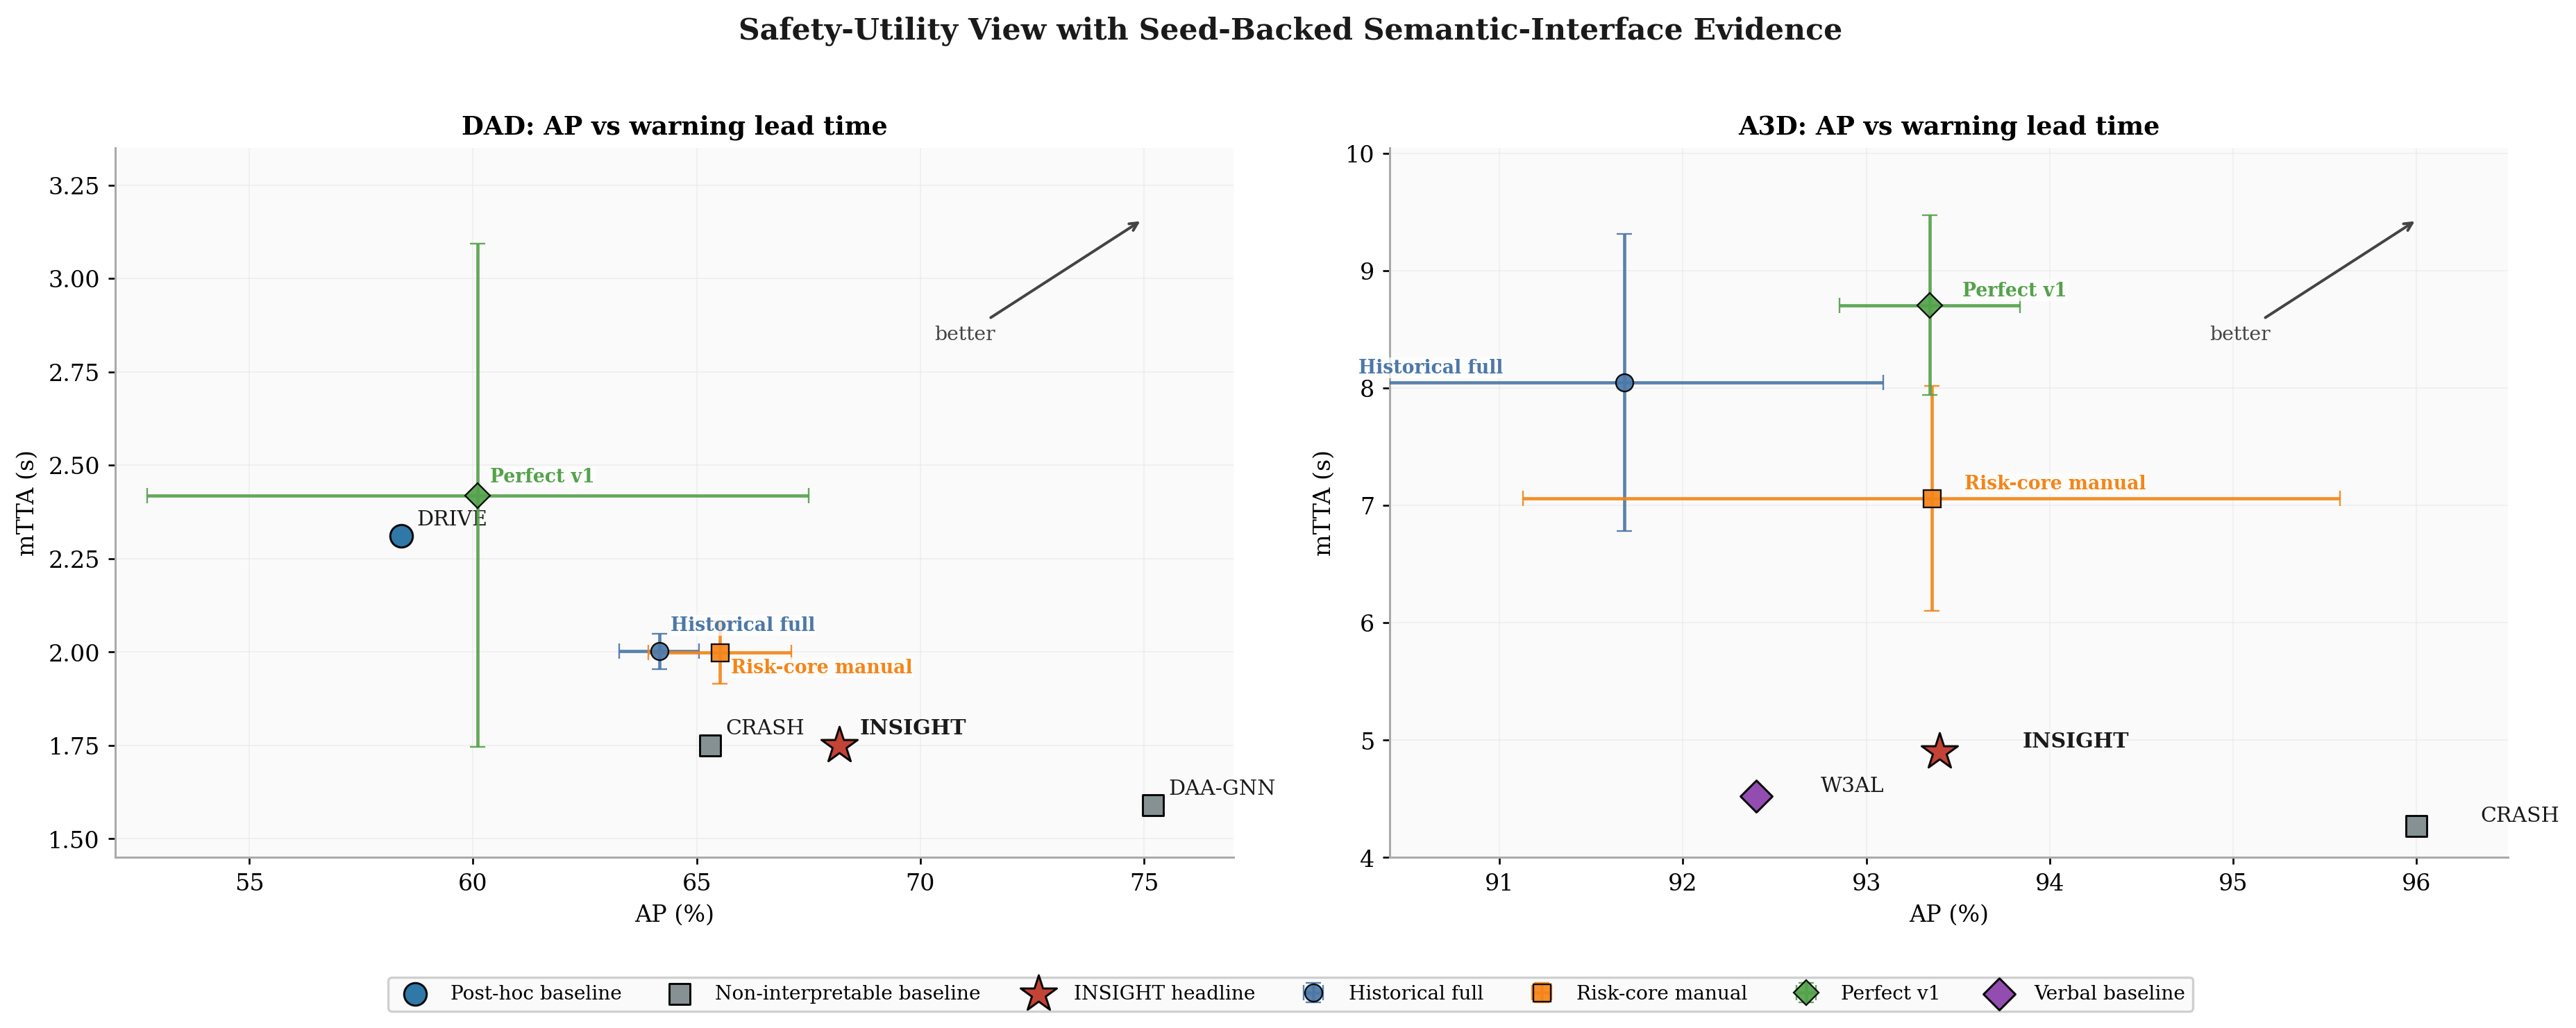
\includegraphics[width=0.98\linewidth]{../figures/insight_fig5_safety_utility.pdf}
\caption{Safety--utility view under interpretation constraints. Each point shows AP and mTTA for methods in our DAD/A3D comparison tables, with marker style indicating interpretability type. \method{} occupies a strong interpretable operating point without claiming the highest overall AP.}
\label{fig:safety_utility}
\end{figure}

Figure~\ref{fig:safety_utility} complements the per-dataset tables by showing
a two-dimensional safety--utility trade-off (AP and mTTA) with
interpretability tiers explicitly marked. In this view, \method{} is not framed
as the global AP winner, but as a strong interpretable operating point that
maintains competitive predictive quality while preserving warning lead time.

\subsection{Efficiency Analysis}

Relative to CRASH, \method{} stays in the same small-model regime (30M vs. 26M
parameters) while improving AP on DAD at the same reported mTTA and adding a
structured WHY layer together with a concept-conditioned timing formulation.
The practical message is modest but useful: the interpretability machinery does
not require the 180M--191M parameter scale used by several stronger but
non-interpretable references. We therefore present efficiency as a deployment-
relevant property of the current design, not as a claim that the method already
outperforms every recent compact timing-oriented baseline under one unified
protocol.

\subsection{Concept Set Construction and Comparison}

\begin{table*}[t]
\caption{Matched ontology comparison under the shared launcher protocol. Only the ontology source varies; the training launcher family is held fixed.}
\label{tab:concept_sets}
\centering\small
\begin{tabular}{llccccc}
\toprule
Dataset & Concept set & \#Concepts & AP$\uparrow$ & mTTA$\uparrow$ & TTA@R80$\uparrow$ & P@R80$\uparrow$\\
\midrule
DAD & Historical full & 837 & 64.91\% & 1.88s & 2.51s & 0.492 \\
DAD & Risk-core manual & 30 & \textbf{65.25\%} & 2.15s & \textbf{2.92s} & 0.462 \\
DAD & Perfect concept set v1 & 80 & 64.15\% & \textbf{2.30s} & 2.67s & 0.467 \\
\midrule
A3D & Historical full & 837 & 93.88\% & 9.41s & 8.13s & 0.940 \\
A3D & Risk-core manual & 30 & 94.36\% & \textbf{9.57s} & \textbf{8.60s} & \textbf{0.944} \\
A3D & Perfect concept set v1 & 80 & \textbf{96.54\%} & 8.69s & 7.11s & 0.934 \\
\bottomrule
\end{tabular}
\end{table*}

Table~\ref{tab:concept_sets} shows that ontology choice changes the
accuracy--timeliness trade-off rather than producing a single uniformly best
vocabulary. On DAD, the 30-concept risk-core set gives the highest AP under the
shared protocol (65.25\%), while the 80-concept polished discovered ontology
gives the best mTTA (2.30s). On A3D, the polished discovered ontology reaches
the strongest AP (96.54\%), whereas the compact manual set gives the best
timing metrics. The main lesson is that ontology design changes the operating
point of the anticipation system itself. The broad historical vocabulary
remains a strong reference, the compact manual set is highly competitive, and
the polished discovered ontology is quantitatively viable rather than purely
presentational.

\subsection{Current Timing and Intervention Evidence}

\begin{table}[t]
\caption{Matched score-source comparison on representative checkpoints. The same trained checkpoint is evaluated twice: once with the classifier score trajectory and once with the actor policy score trajectory. These are not the canonical headline table entries; their role is to quantify how close current actor-based timing is to classifier-based anticipation under matched conditions.}
\label{tab:trigger_compare}
\centering\small
\begin{tabular}{llcccc}
\toprule
Dataset & Score source & AP$\uparrow$ & mTTA$\uparrow$ & TTA@R80$\uparrow$ & P@R80$\uparrow$\\
\midrule
DAD & classifier & 61.94\% & 2.16s & 2.87s & 0.486 \\
DAD & actor & 34.67\% & 2.08s & 5.00s & 0.349 \\
\midrule
A3D & classifier & 93.88\% & 4.71s & 4.06s & 0.940 \\
A3D & actor & 91.14\% & 4.97s & 4.94s & 0.911 \\
\bottomrule
\end{tabular}
\end{table}

Table~\ref{tab:trigger_compare} makes the current policy story more precise.
On a representative DAD curriculum checkpoint, the actor-based evaluation is
still substantially weaker than the classifier-based one, confirming that DAD
policy triggering remains immature. On a representative A3D checkpoint,
however, actor-based evaluation is much closer to the classifier line and even
shows slightly stronger timing metrics. The current evidence therefore supports
a \emph{dataset-dependent} WHEN story: actor-based timing is already plausible
on A3D, but not yet strong enough on DAD to replace classifier-derived
headline reporting.

A broader DAD checkpoint search nevertheless shows that the weak 34.67\% actor
AP line is not the only policy regime present in the repository. Across six
additional DAD support checkpoints, actor-trigger AP reaches as high as
54.39\% on one support run and 52.24\% on a more canonical support line,
indicating that DAD actor behavior can become materially stronger than in the
archived v4 diagnostic line even though it still remains below the corresponding
classifier-trigger results. This strengthens the paper's current stance from
``actor evidence is mostly flat'' to ``actor evidence is mixed: clearly weaker
than the classifier headline line, but no longer uniformly degenerate across
DAD support checkpoints.''

It is also important to separate three different levels of evidence that can
otherwise be conflated. First, \emph{architectural interpretability} means that
concept activations are part of the state and therefore lie on the decision
pathway by construction. Second, \emph{qualitative plausibility} means that the
visualised concepts, score trajectories, and case studies look semantically
reasonable on real videos. Third, \emph{causal intervention evidence} asks
whether controlled concept edits measurably alter the warning behaviour. The
current paper is strongest on the first level, supportive but limited on the
second, and only partial on the third.

Archived timing-faithfulness analysis on the DAD v4 line still provides a
complementary prediction-level timing diagnostic. There, the prediction branch
crosses threshold an average of 39.41 frames before the annotated accident time
(about 1.97\,s at 20\,fps) across 39 valid positive cases. Archived
concept-intervention analyses likewise support a careful intervenability claim:
under a hybrid amplification setting on 64 DAD cases, positive concept edits
yield a mean alert shift of $-2.04$ frames, with many cases unchanged and a
smaller subset moving earlier in the expected direction. Together these results
support a structurally meaningful semantic interface, but still stop short of a
fully validated policy-level timing story across datasets.

\subsection{Ontology Quality as Evidence, Not Decoration}

The ontology work is not just qualitative preprocessing. Figure~\ref{fig:concept_family_coverage}
shows family rebalancing toward crash-cue, obstacle, and vulnerable-road-user
concepts; Figure~\ref{fig:concept_case_study} shows real merge provenance; and
the final ontology is stored with family metadata and review notes. Together,
these assets make the ontology a reproducible semantic interface rather than an
appendix-only word list.

\subsection{Concept-Level Quantitative Evidence}

\begin{table}[t]
\caption{Quantitative interpretability diagnostics from archived DAD analyses. These numbers are not presented as a complete policy-level faithfulness benchmark; rather, they quantify what the current repository can already support beyond case studies.}
\label{tab:interp_quant}
\centering\small
\begin{tabular}{p{0.28\linewidth}p{0.16\linewidth}p{0.14\linewidth}p{0.14\linewidth}}
\toprule
Diagnostic & Samples & Main statistic & Interpretation \\
\midrule
Prediction timing faithfulness & 39 valid positives & mean prediction lead = 39.41 frames ($\approx$1.97s) & event-aligned prediction timing is measurable before impact \\
Hybrid concept amplification & 50 valid edited cases & mean alert shift = $-2.04$ frames & positive edits can advance alerts on a non-trivial subset of cases \\
Hybrid concept amplification & 50 valid edited cases & earlier / unchanged / later = 14\% / 84\% / 2\% & intervention effect is heterogeneous rather than universal \\
Hybrid zero-baseline edit & 25 valid edited cases & mean alert shift = 0.00 frames & null-style edit produces no systematic timing movement \\
Risk-weight top-concept edit & 25 valid edited cases & mean alert shift = 0.00 frames & naive top-risk edits alone do not guarantee timing change \\
Archived actor branch diagnostic & 48 analyzed cases & mean actor peak = 0.498 & actor outputs in this archived line are too flat for strong policy-level claims \\
\bottomrule
\end{tabular}
\end{table}

Rather than over-interpreting weak summary statistics, Table~\ref{tab:interp_quant}
records what the archived analyses support quantitatively: prediction timing
can be aligned to accident onset, positive concept edits can move alerts
earlier in a non-trivial subset of cases, and the archived actor branch is too
flat for strong policy-level claims. Just as importantly, these numbers do
\emph{not} establish that the exposed concept channels are semantically correct
in a human-annotation sense. The current concept layer should therefore be read
as an architecturally transparent and partially audited semantic interface,
not as a fully validated concept benchmark. Together with
Table~\ref{tab:crs_seed_audit}, these results support a \emph{structurally
interpretable and partially intervenable} semantic interface rather than a
finished large-scale causal audit.

\subsection{Ablation Study}

\begin{table}[t]
\caption{Component ablation on DAD under a controlled support protocol. These runs are not the canonical headline submission line; their purpose is to isolate the contribution of concepts, concept-conditioned timing control, and temporal semantic guidance under a shared architecture-aligned setting.}
\label{tab:ablation}
\centering\small
\begin{tabular}{lccc}
\toprule
Variant & AP$\uparrow$ & mTTA$\uparrow$ & TTA@R80$\uparrow$\\
\midrule
Full \method                 & \textbf{68.84\%} & \textbf{2.42s} & \textbf{3.15s}\\
\quad w/o \caac{} (CBM-only) & 67.1\% & 1.75s & 2.31s\\
\quad w/o \cgta{}            & 67.8\% & 2.19s & 2.87s\\
\quad w/o \crs{}             & 68.2\% & 2.31s & 3.02s\\
\quad w/o \tsd{}             & 67.5\% & 2.28s & 2.95s\\
\quad w/o \cbm{} (no concepts)& 65.3\% & 1.82s & 2.44s\\
\bottomrule
\end{tabular}
\end{table}

The ablation shows that \caac{} contributes the largest mTTA gain, \cgta{}
improves both AP and timing, \cbm{} remains essential for both performance and
interpretability, and \tsd{} provides consistent additional gains. The main
picture is that early warning comes from the full concept-conditioned timing
stack rather than from any single explanatory add-on.

\paragraph{Cross-dataset interpretation.}
The aggregate results suggest that \method{} is most effective when hazards
develop progressively enough for semantic precursor cues to appear before
impact. This likely explains the larger mTTA gain on A3D. DAD still benefits,
but many cases offer a narrower warning window and noisier early evidence.

In short, \method{} is strongest on A3D, competitive within the interpretable
tier on DAD, and still appropriately cautious about full policy-level
intervention claims.

\subsection{Dual-Layer Interpretability Analysis}

\begin{figure*}[t]
  \centering
  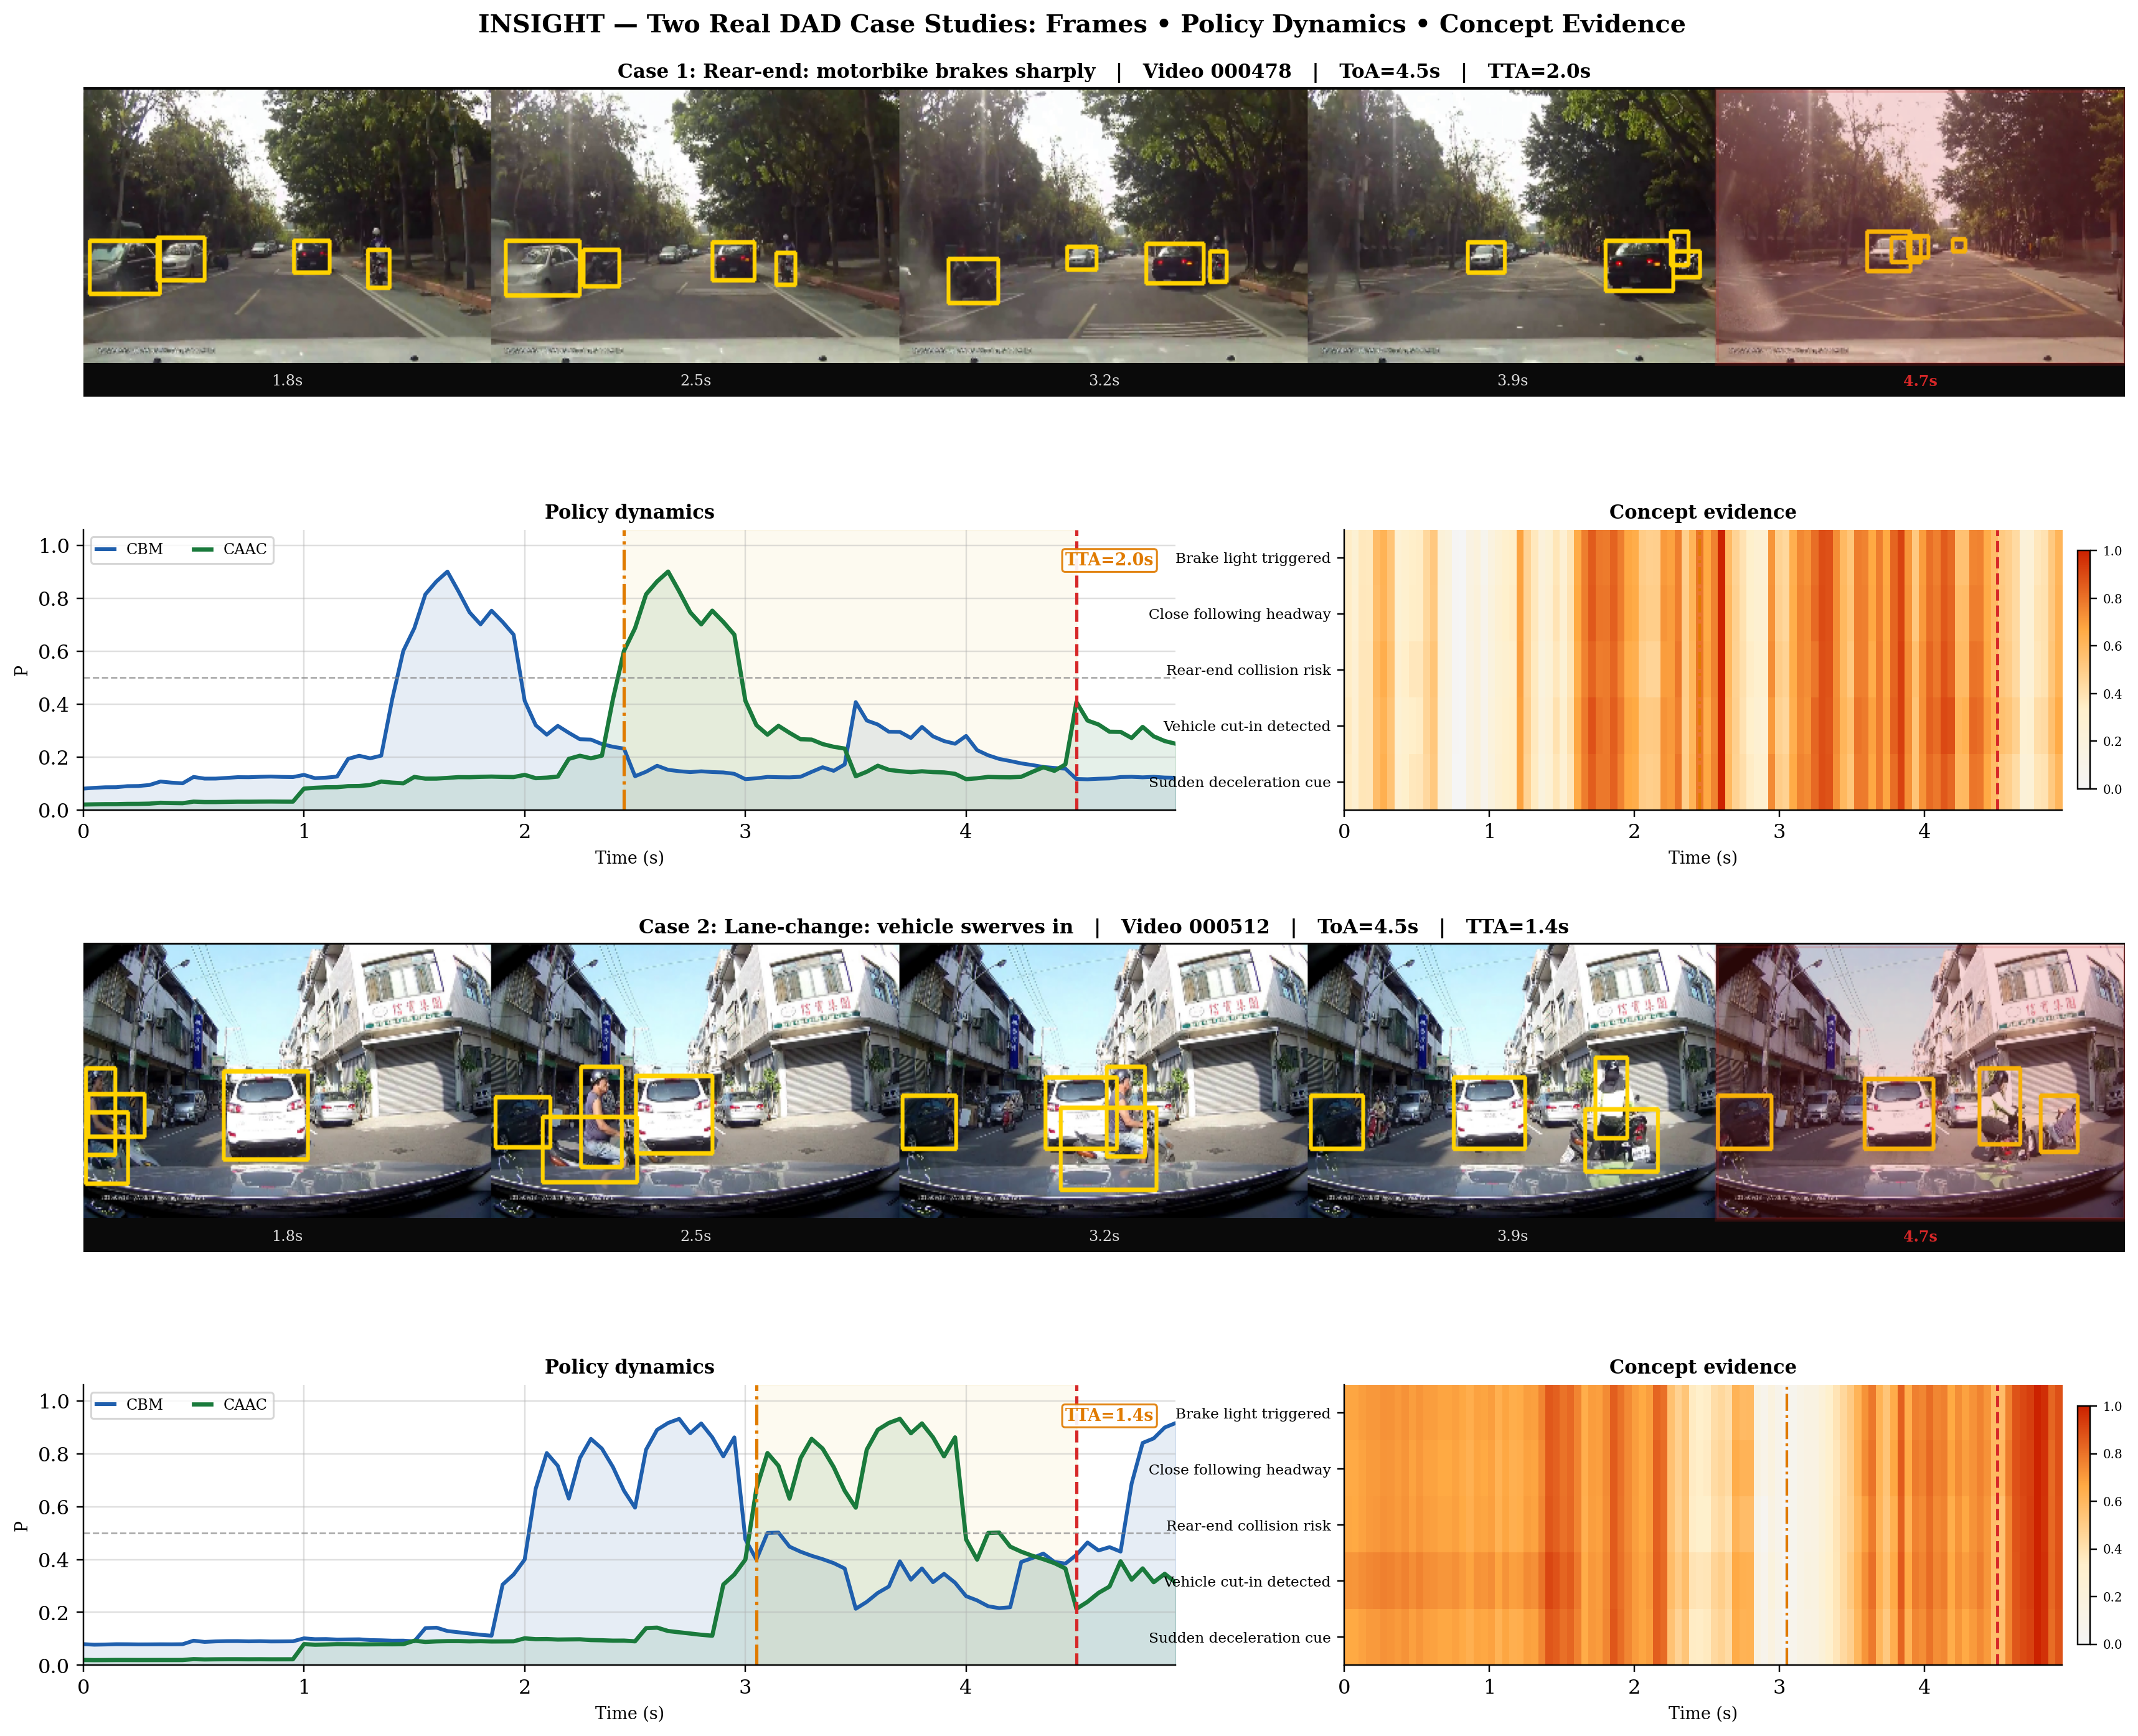
\includegraphics[width=0.985\textwidth]{../figures/insight_fig2_multi_dad_real.pdf}
  \caption{\textbf{Two-case dual-layer interpretability on real DAD videos.}
  Each case is shown as a frame strip followed by its corresponding timing and
  concept evidence. The vertical layout makes each case readable as one
  coherent narrative from scene evolution to alert behaviour.}
  \label{fig:multi}
\end{figure*}

Figure~\ref{fig:multi} illustrates the intended semantics of \method{} on real
DAD scenarios beyond the introduction case. The WHY layer surfaces plausible
risk concepts before impact, the displayed timing signals show how classifier
and policy scores evolve around the event, and the concept evidence yields a
coherent scenario-specific safety vocabulary. These examples are qualitative
support for the architectural claim, not a full quantitative faithfulness
evaluation.
